\documentclass[12pt,a4paper,draft]{ctexart}
\usepackage[utf8]{inputenc}
\usepackage{amsmath}
\usepackage{amsfonts}
\usepackage{amssymb}
\usepackage{graphicx}
\usepackage{bm}
\usepackage[backend=biber,backref=true%nature,% citestyle=gb7714−2015,backref=true%
]{biblatex}
%参考文献数据源加载 
\addbibresource[location=local]{ref.bib}
%\usepackage[left=3.0cm, right=3.0cm, top=3.5cm, bottom=2.70cm]{geometry}
\title{隐马尔科夫模型 \\
	在拼音输入法中的应用研究}
\author{Yuan}
\date{\small\today}
\begin{document}

\maketitle
\begin{abstract}
本文尝试将隐马尔科夫模型应用于中文整句拼音输入中,给出了具体的模型和实际问题的对应关系以及参数估计的方法。同时还选用了现有的中文语料库进行了实现,取得了较好的效果。
\end{abstract}	
\section{引言}
隐马尔科夫模型(Hidden Markov Model,HMM)是一种应用于序列问题的统计学系模型,该模型描述了由隐藏的马尔科夫链随机生成观测序列的过程。HMM非常适合解决标注问题,故HMM在语音识别、自然语言处理、生物信息、模式识别等领域有广泛的应用,本文着眼于将HMM应用于中文拼音输入法。拼音输入法将拼音转换为对应汉字,其中更具有实用价值的是将连续的拼音输入转换为连续的句子。这是典型的序列问题,更为具体地,是一种序列标注问题,故应用HMM能较好的解决该问题。
\section{问题描述}
HMM描述了一个隐藏的马尔科夫链生成不可观测的状态随机序列,再由各个状态生成一个观测而产生观测随机序列的过程。HMM随机生成的状态序列成为状态序列(state sequence);每一个状态生成一个观测,而由此产生的观测的随机序列成为观测序列(observation sequence)。故HMM可以由初始概率分布、状态转移概率分布以及观测概率分布确定,这三者对应的参数分别为初始状态概率向量$ \bm{\pi} $、状态转移概率矩阵$\bm{A}$及观测概率矩阵$\bm{B}$。由此HMM可以用三元组$ \lambda=(\bm{A},\bm{B},\bm{\pi}) $表示\cite{李航统计学习}。
\subsection{模型定义}
在拼音序列转汉字的问题中,连续的句子被视为序列,即认为每个时刻对应一个汉字,汉字又对应拼音。由于用户在输入法中输入的是拼音,所以拼音序列被定义为观测序列。而汉字则为生成观测序列的状态序列。故本应用下的HMM相关定义为:


所有的汉字组成集合Q(状态集合),所有汉字对应的拼音的集合V(观测集合),其中$ |Q|=N, |V|=M $。
\[ Q=\{ \mbox{汉字}_1,\mbox{汉字}_2,\cdots,\mbox{汉字}_N \},V=\{ \mbox{拼音}_1,\mbox{拼音}_2,\cdots,\mbox{拼音}_M \}  \]

用户想输入的汉字序列I(状态序列),用户实际输入的拼音序列O(观测序列),其中$ |I|=|O|=T $。
\[ I=\{ \mbox{预期汉字}_1,\mbox{预期汉字}_2,\cdots,\mbox{预期汉字}_T \}	\]
\[O=\{ \mbox{输入拼音}_1,\mbox{输入拼音}_2,\cdots,\mbox{输入拼音}_T \}  \]

句子中前后汉字转移概率矩阵$\bm{A}$:
\[ \bm{A}=[a_{ij}]_{N\times N} \]
其中,
\[ a_{ij}=P(i_{t+1}=\mbox{汉字}_j|i_t=\mbox{汉字}_i),  i=1,2,3,\cdots,N; j=1,2,\cdots,N\]
是在句子中的位置$ t $处的$ \mbox{汉字}_i $转移到$ t+1 $处的$ \mbox{汉字}_j $的概率。
句子中前后汉字转移概率矩阵$\bm{B}$:
\[ \bm{B}=[b_j(k)]_{N\times M} \]
其中,
\[ b_j(k)=P(\mbox{t处输入的拼音}=\mbox{拼音}_k|\mbox{ t处想要输入的汉字}=\mbox{汉字}_j) \]
\[ k=1,2,3,\cdots,M; j=1,2,\cdots,N\]
是在句子中的位置$ t $处的$ \mbox{汉字}_j $生成$ \mbox{拼音}_k $的概率。

句子中首个汉字出现可能性的概率向量$\bm{\pi}$:
\[ \bm{\pi}=(\pi_i) \]
其中,
\[ \pi_i=P(\mbox{句首汉字}=\mbox{汉字}_i), i=1,2,\cdots,N \]
是句首汉字为$\mbox{汉字}_i$的概率。
\subsection{模型训练(参数估计)}
HMM的训练可以采用监督学习或者无监督学习\cite{李航统计学习},本应用的状态和观测为汉字和拼音。将汉字转化为拼音可以自动开展\cite{python-pinyin},并有相当高的准确度\cite{accuracy-of-auto-pinyin}。故可以通过中文语料库生成用于监督学习的训练集。
本应用中HMM的三元组$ \lambda=(\bm{A},\bm{B},\bm{\pi}) $的估计方法如下:
\paragraph{前后汉字转移概率$a_{ij}$的估计}
\[ \hat{a}_{i j}=\frac{A_{ij}}{\sum_{j=1}^{N} A_{i j}}, \quad i=1,2, \cdots, N ; j=1,2, \cdots, N \]
\paragraph{汉字转拼音的概率$b_j(k)$的估计}
\[ \hat{b}_{j}(k)=\frac{B_{j k}}{\sum_{k=1}^{M} B_{j k}}, \quad j=1,2, \cdots, N ; k=1,2, \cdots, M \]
\paragraph{句首汉字出现概率$\pi_i$的估计}


\section{实验}
参数估计使用的语料源自搜狗实验室提供的搜狐往年的新闻数据集\cite{SogouCS}。原始的数据集非常庞大,通过清洗整理后得到如表x所述的数据集。


\begin{figure}
	\centering
	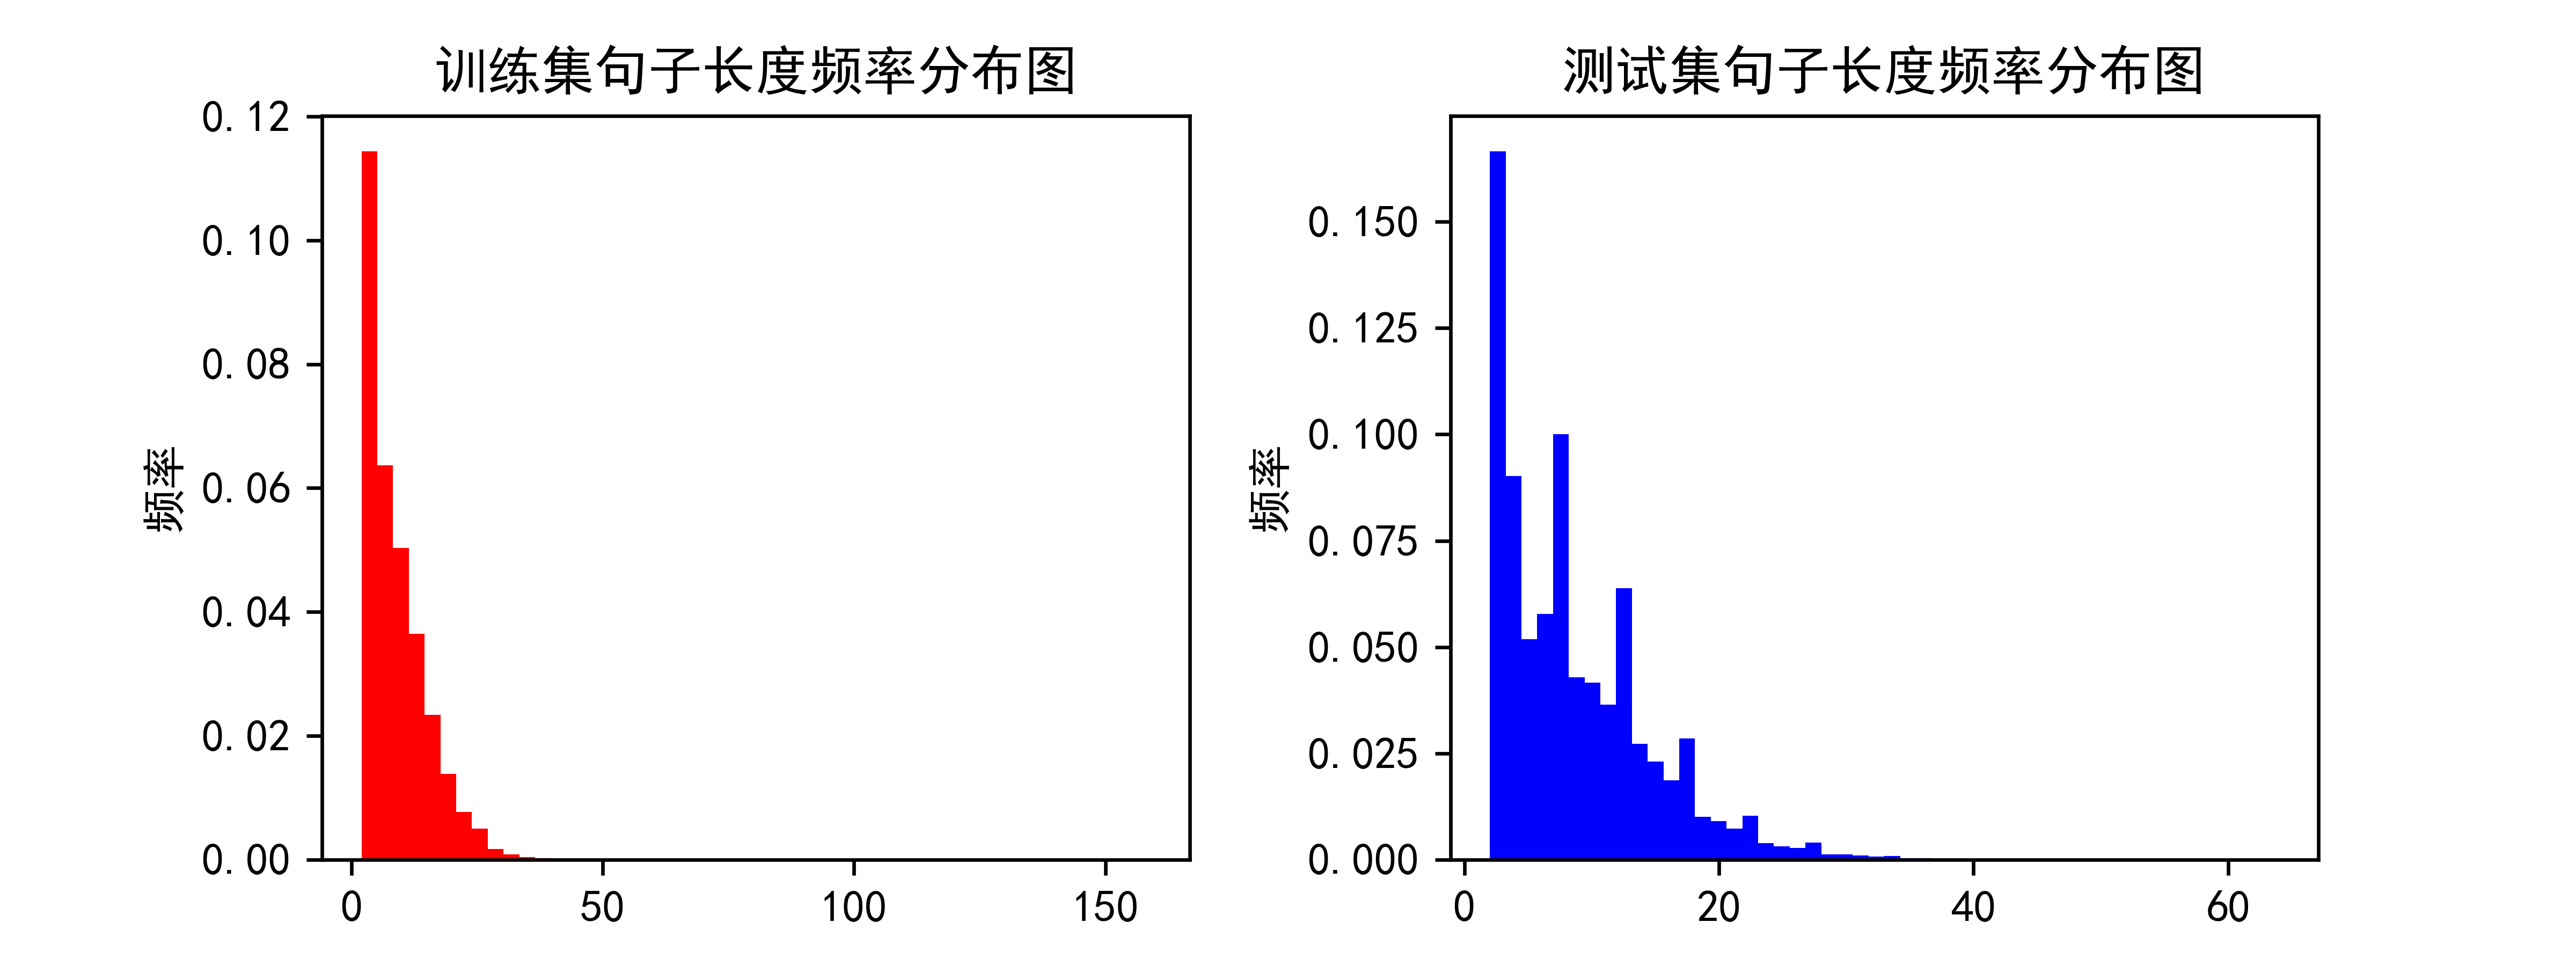
\includegraphics[width=1\linewidth]{DataSetHistogram}
	\caption{}
	\label{fig:datasethistogram}
\end{figure}




\printbibliography[heading=bibliography,title=参考文献]
\end{document}